\ifdefined\COMPLETE
\else
\documentclass[12pt]{article}
\usepackage{tikz}
\usetikzlibrary{shapes, calc, arrows, through, intersections, decorations.pathreplacing, patterns}

\begin{document}
\fi

\def\alph{$2+\sqrt{5}$}
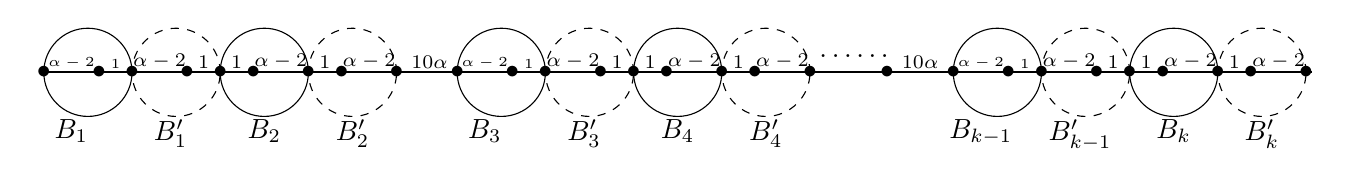
\begin{tikzpicture}[scale=7]

	\coordinate (x) at ($ (-0.10,{sqrt(0)}) $);
	\coordinate (y) at (2.2,0);
	\draw[thick] (x) --(y);

	\node[] at (-0.10,0) {$\bullet$};
	\node[label={[yshift=-0.2cm]\tiny $\alpha-2$}] at (-0.05,0) {};
	\node[] at (0.0,0) {$\bullet$};
	\node[label={[yshift=-0.2cm]\tiny $1$}] at (0.03,0) {};
	\node[] at (0.06,0) {$\bullet$};
	\node[label={[yshift=-0.2cm]\scriptsize $\alpha-2$}] at (0.11,0) {};
	\node[] at (0.16,0) {$\bullet$};
	\node[label={[yshift=-0.2cm]\scriptsize $1$}] at (0.19,0) {};
	\node[] at (0.22,0) {$\bullet$};
	\node[label={[yshift=-0.2cm]\scriptsize $1$}] at (0.25,0) {};
	\node[] at (0.28,0) {$\bullet$};
	\node[label={[yshift=-0.2cm]\scriptsize $\alpha-2$}] at (0.33,0) {};
	\node[] at (0.38,0) {$\bullet$};
	\node[label={[yshift=-0.2cm]\scriptsize $1$}] at (0.41,0) {};
	\node[] at (0.44,0) {$\bullet$};	
	\node[label={[yshift=-0.2cm]\scriptsize $\alpha-2$}] at (0.49,0) {};
	\node[] at (0.54,0) {$\bullet$};	
	\node[label={[yshift=-0.2cm]\scriptsize $10\alpha$}] at (0.6,0) {};
	
	
	\node[] at (0.65,0) {$\bullet$};
	\node[label={[yshift=-0.2cm]\tiny $\alpha-2$}] at (0.7,0) {};
	\node[] at (0.75,0) {$\bullet$};
	\node[label={[yshift=-0.2cm]\tiny $1$}] at (0.78,0) {};
	\node[] at (0.81,0) {$\bullet$};
	\node[label={[yshift=-0.2cm]\scriptsize $\alpha-2$}] at (0.86,0) {};
	\node[] at (0.91,0) {$\bullet$};
	\node[label={[yshift=-0.2cm]\scriptsize $1$}] at (0.94,0) {};
	\node[] at (0.97,0) {$\bullet$};
	\node[label={[yshift=-0.2cm]\scriptsize $1$}] at (1.0,0) {};
	\node[] at (1.03,0) {$\bullet$};
	\node[label={[yshift=-0.2cm]\scriptsize $\alpha-2$}] at (1.08,0) {};
	\node[] at (1.13,0) {$\bullet$};
	\node[label={[yshift=-0.2cm]\scriptsize $1$}] at (1.16,0) {};
	\node[] at (1.19,0) {$\bullet$};	
	\node[label={[yshift=-0.2cm]\scriptsize $\alpha-2$}] at (1.24,0) {};
	\node[] at (1.29,0) {$\bullet$};	
	
	
	
	\node[] at (1.37,0.03) {$\ldots\ldots$};
	\node at (1.43,0.0) {$\bullet$};	
	\node[label={[yshift=-0.2cm]\scriptsize $10\alpha$}] at (1.49,0) {};
	
	\node[] at (1.55,0) {$\bullet$};
	\node[label={[yshift=-0.2cm]\tiny $\alpha-2$}] at (1.6,0) {};
	\node[] at (1.65,0) {$\bullet$};
	\node[label={[yshift=-0.2cm]\tiny $1$}] at (1.68,0) {};
	\node[] at (1.71,0) {$\bullet$};
	\node[label={[yshift=-0.2cm]\scriptsize $\alpha-2$}] at (1.76,0) {};
	\node[] at (1.81,0) {$\bullet$};
	\node[label={[yshift=-0.2cm]\scriptsize $1$}] at (1.84,0) {};
	\node[] at (1.87,0) {$\bullet$};
	\node[label={[yshift=-0.2cm]\scriptsize $1$}] at (1.9,0) {};
	\node[] at (1.93,0) {$\bullet$};
	\node[label={[yshift=-0.2cm]\scriptsize $\alpha-2$}] at (1.98,0) {};
	\node[] at (2.03,0) {$\bullet$};
	\node[label={[yshift=-0.2cm]\scriptsize $1$}] at (2.06,0) {};
	\node[] at (2.09,0) {$\bullet$};	
	\node[label={[yshift=-0.2cm]\scriptsize $\alpha-2$}] at (2.14,0) {};
	\node[] at (2.19,0) {$\bullet$};
	
	
	
	\node[label=270:$B_1$] at (-0.05,-0.05) {};	
	\node[label=270:$B_1'$] at (0.13,-0.05) {};	
	\node[label=270:$B_2$] at (0.3,-0.05) {};	
	\node[label=270:$B_2'$] at (0.46,-0.05) {};
	
	\node[label=270:$B_3$] at (0.7,-0.05) {};	
	\node[label=270:$B_3'$] at (0.88,-0.05) {};	
	\node[label=270:$B_4$] at (1.05,-0.05) {};	
	\node[label=270:$B_4'$] at (1.21,-0.05) {};
	
	\node[label=270:$B_{k-1}$] at (1.6,-0.05) {};	
	\node[label=270:$B_{k-1}'$] at (1.78,-0.05) {};	
	\node[label=270:$B_{k}$] at (1.95,-0.05) {};	
	\node[label=270:$B_k'$] at (2.11,-0.05) {};
	
	
	\draw (-0.02,0) circle (0.08) ;
	\draw[dashed] (0.14,0) circle (0.08);
	\draw (0.3,0) circle (0.08cm);
	\draw[dashed] (0.46, 0.0) circle (0.08) ;
	
	\draw (0.73,0) circle (0.08) ;
	\draw[dashed] (0.89,0) circle (0.08);
	\draw (1.05,0) circle (0.08cm);
	\draw[dashed] (1.21, 0.0) circle (0.08) ;
	
	\draw (1.63,0) circle (0.08) ;
	\draw[dashed] (1.79,0) circle (0.08);
	\draw (1.95,0) circle (0.08cm);
	\draw[dashed] (2.11, 0.0) circle (0.08) ;
	%\draw (A) -- (1.74, 0.06);
\end{tikzpicture}


\ifdefined\COMPLETE
\else
\end{document}
\fi
